\chapter{E--pH 图}\label{ch:b1:e-ph-diagrams}

放在雨水中的铁钉会生锈；同一枚铁钉
浸在\omterm{def:b1:predominant-reaction:strong-acid}{强碱}性溶液中，数周仍保持光泽。船体钢板上装有锌块，
锌块代替钢板溶解，而铜屋顶
会变绿，却从不消失。电势随 pH 而变的\omterm{def:b1:nernst:couple}{氧化还原电对}、
氢氧化物与氧化物的沉淀、酸碱平衡：三者同时起作用，
而一张图即可将它们汇总。在电势对 pH 的图上，
元素的每种物种都占有一个区域，即它为稳定形式的区域；
读图即可知道哪些物种能在水中存留、哪些物种会相互反应，
以及金属在何处发生腐蚀。

\begin{recall}
\omterm{thm:b1:nernst:nernst}{能斯特方程}、标准电势以及氧化还原反应的预测，
见\cref{ch:b1:nernst}；\omterm{def:b1:predominant-reaction:predominance}{优势区域图}
见\cref{ch:b1:predominant-reaction}；氢氧化物的沉淀阈值
与固体的\omterm{def:b1:precipitation:existence-domain}{存在区域}见\cref{ch:b1:precipitation}。
所有电势均在 \qty{25}{\celsius} 下取值，且 $RT\ln 10/F = \qty{0.059}{V}$。
\end{recall}

\begin{omfigure}
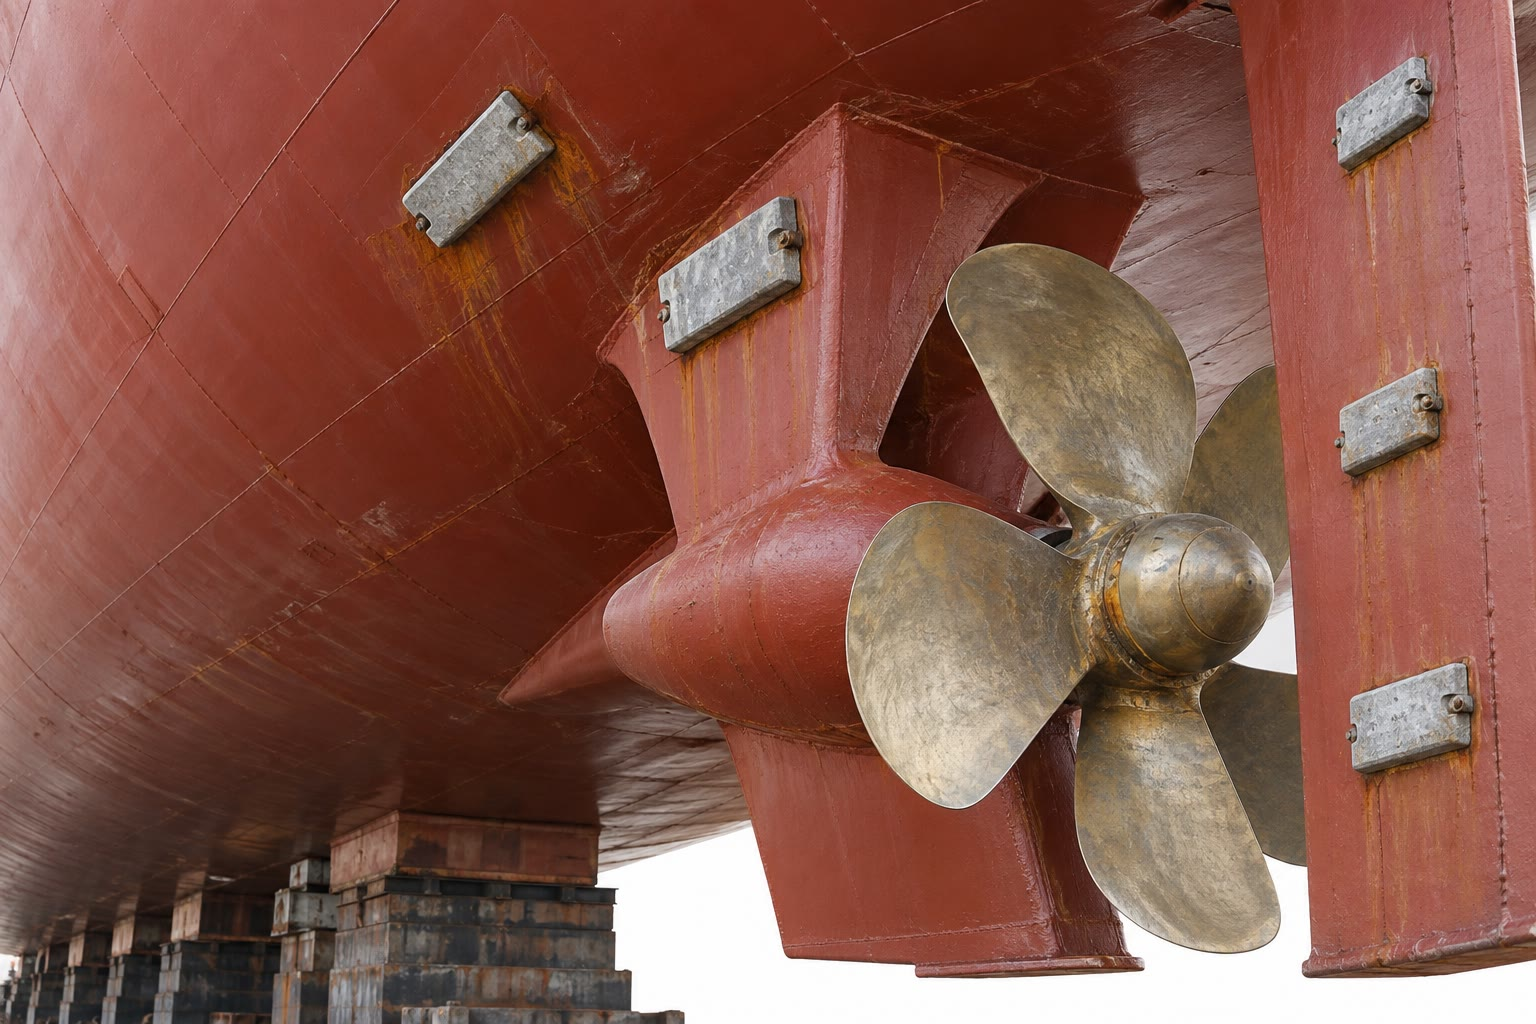
\includegraphics[width=0.6\linewidth]{images/book2/ai/b1-14-ship-anodes.jpg}

{\small 干船坞中一艘船的船尾。固定在船体上的灰色块，
靠近螺旋桨的为锌块：在海水中，它们代替
钢板而发生腐蚀（见\cref{exo:b1:e-ph-diagrams:12}）。}
\end{omfigure}

\section{约定}

\begin{definition}[电势--pH 图，边界浓度]\label{def:b1:e-ph-diagrams:e-ph-diagram}
某元素的\emph{电势--pH 图}\index{电势--pH 图}是平面 $(\mathrm{pH}, E)$
被划分为若干区域，每个区域为
该元素某一种形式的优势区域（溶解态物种）或\omterm{def:b1:precipitation:existence-domain}{存在区域}（固体）。
绘制时取定一个\emph{边界
浓度}\index{边界浓度} $c$，即溶液中该元素的总浓度，
并采用以下约定：
\begin{itemize}
  \item 在两种溶解态物种之间的边界上，两者的浓度均为 $c$
        （以该元素的原子计）；
  \item 在溶解态物种与固体之间的边界上，
        溶解态物种的浓度为 $c$，固体仅需存在；
  \item 气体的压强为 \qty{1}{bar}。
\end{itemize}
本章中 $c = \qty{0.010}{mol/L}$。
\end{definition}

元素的各种形式按\omterm{def:b1:nernst:oxidation-number}{氧化数}排序：\omterm{def:b1:nernst:oxidation-number}{氧化数}越高，
在图中位置越靠上（氧化态形式
在较高电势下稳定）。在\omterm{def:b1:nernst:oxidation-number}{氧化数}相同时，碱性较强的形式
（氢氧化物、氧化物、羟基\omterm{def:b1:complexation:complex}{配合物}）位于右侧。

\begin{proposition}[边界的斜率]\label{prop:b1:e-ph-diagrams:boundary-slope}
两种\omterm{def:b1:nernst:oxidation-number}{氧化数}不同的物种之间的边界，其半反应
交换 $n$ 个电子和 $m$ 个质子，
$\mathrm{Ox} + m\,\ce{H+} + n\,\mathrm{e^-} \rightleftharpoons \mathrm{Red} +
\cdots$，则该边界为斜率为 $-0.059\,m/n$ 伏特每 pH 单位的直线。
两种\omterm{def:b1:nernst:oxidation-number}{氧化数}相同的物种之间的边界为竖直线。
\end{proposition}

\begin{proof}
由\omterm{thm:b1:nernst:nernst}{能斯特方程}得 $E = E^\circ + \frac{0.059}{n}\log\frac{[\mathrm{Ox}]
[\ce{H+}]^m}{[\mathrm{Red}]} = E^\circ + \frac{0.059}{n}\log\frac{[\mathrm{Ox}]}
{[\mathrm{Red}]} - \frac{0.059\,m}{n}\,\mathrm{pH}$，而边界上的
浓度由约定确定。\omterm{def:b1:nernst:oxidation-number}{氧化数}相同的两种物种
通过酸碱平衡或沉淀平衡相联系，
不涉及电子，其平衡常数决定边界的 pH，
与电势无关。
\end{proof}

\section{水}

\begin{proposition}[水的两条线]\label{prop:b1:e-ph-diagrams:water-lines}
在 \qty{1}{bar} 的气体压强下，水在
直线 $E = -0.059\,\mathrm{pH}$ 以下被还原为氢气，在直线 $E = 1.23
- 0.059\,\mathrm{pH}$ 以上被氧化为氧气。
\end{proposition}

\begin{proof}
\ce{2H+ + 2e- -> H2}：$E = 0 + \frac{0.059}{2}\log\frac{[\ce{H+}]^2}{p(\ce{H2})}
= -0.059\,\mathrm{pH}$（$p = 1$ 时）。\ce{O2 + 4H+ + 4e- -> 2H2O}：$E = 1.23 +
\frac{0.059}{4}\log(p(\ce{O2})[\ce{H+}]^4) = 1.23 - 0.059\,\mathrm{pH}$。在
第一条线以下，\ce{H2} 是该电对的稳定形式（水被还原）；
在第二条线以上，\ce{O2} 是稳定形式。
\end{proof}

\begin{definition}[水的稳定区]\label{def:b1:e-ph-diagrams:water-domain}
两条线之间的区带，在每个 pH 下宽度均为 \qty{1.23}{V}，称为
\emph{水的稳定区}\index{水的稳定区}：区域完全位于该区带之内的
物种，既不氧化水，
也不还原水。
\end{definition}

\section{绘制图：铁}

\begin{method}[绘制电势--pH 图]\label{met:b1:e-ph-diagrams:build}
\begin{enumerate}
  \item 列出各物种，并按\omterm{def:b1:nernst:oxidation-number}{氧化数}排序：对铁而言，
        \ce{Fe}（0）、\ce{Fe^2+} 与 \ce{Fe(OH)2}（$+$II）、\ce{Fe^3+} 与
        \ce{Fe(OH)3}（$+$III）。
  \item 在每个\omterm{def:b1:nernst:oxidation-number}{氧化数}下，依
        \omterm{def:b1:e-ph-diagrams:e-ph-diagram}{边界浓度}下的沉淀（或酸碱）平衡求出竖直边界
        （见\cref{ch:b1:precipitation}）。
  \item 对每一对相邻\omterm{def:b1:nernst:oxidation-number}{氧化数}，在各 pH 范围内写出半反应，
        并依约定写出其\omterm{thm:b1:nernst:nernst}{能斯特方程}；
        由此得到斜率已知的直线边界。
  \item 自左至右连接各线段；三线交汇处，
        每条线只延伸到其两种物种都
        稳定的一侧。
  \item 检验：各区域不得重叠，且斜率须与
        \cref{prop:b1:e-ph-diagrams:boundary-slope}相符。
\end{enumerate}
\end{method}

\begin{example}[铁的边界]\label{ex:b1:e-ph-diagrams:iron}
取 $c = \qty{0.010}{mol/L}$（常数取自\cref{ch:b1:precipitation,ch:b1:nernst}）：
\begin{itemize}
  \item \ce{Fe^3+}/\ce{Fe(OH)3}：$\mathrm{pH} = 14.00 - \frac13(38.55 - 2) = 1.82$；
        \ce{Fe^2+}/\ce{Fe(OH)2}：$\mathrm{pH} = 14.00 - \frac12(16.31 - 2) = 6.85$。
  \item \ce{Fe^2+}/\ce{Fe}：$E = -0.41 + 0.030\log c = -0.47$~V（pH 低于 6.85）。
  \item \ce{Fe^3+}/\ce{Fe^2+}：$E = 0.77$~V（两者浓度均为 $c$，pH 低于 1.82）。
  \item \ce{Fe(OH)3}/\ce{Fe^2+}：\ce{Fe(OH)3 + 3H+ + e- -> Fe^2+ + 3H2O}，斜率
        $-0.177$：$E = 1.09 - 0.177\,\mathrm{pH}$，适用于 pH 在 1.82 与 6.85 之间。
  \item \ce{Fe(OH)3}/\ce{Fe(OH)2}：一个电子、一个质子，$E = 0.28 -
        0.059\,\mathrm{pH}$；\ce{Fe(OH)2}/\ce{Fe}：两个电子、两个
        质子，$E = -0.07 - 0.059\,\mathrm{pH}$（pH 高于 6.85）。
\end{itemize}
截距可由三相点处的连续性求得，也可直接由生成吉布斯自由能算出；
下图由后一种方法算得，其边界与
这些取整后的数值相差
不超过 \qty{0.01}{V} 或 0.01 个 pH 单位。
% ledger: dfg:Fe2+_ao, dfg:Fe3+_ao, dfg:Fe_OH2_cr, dfg:Fe_OH3_cr, dfg:H2O_l, dfg:OH-_ao (boundaries computed in figdata/bachelor-1/eph-diagrams.py)
\end{example}

\begin{omfigure}
\begin{tikzpicture}
\begin{axis}[
  width=0.8\linewidth, height=8.2cm, xmin=0, xmax=14, ymin=-1.2, ymax=1.6,
  axis x line=bottom, axis y line=left, xlabel={pH}, ylabel={$E$ (V)},
  xtick={0,2,4,6,8,10,12,14}, ytick={-1,-0.5,0,0.5,1,1.5},
  unbounded coords=jump, clip=true,
  tick label style={font=\small}, label style={font=\small}]
\addplot[black!45, dashed] table[x=pH, y=H2] {figdata/out/bachelor-1-eph-diagrams-water.dat};
\addplot[black!45, dashed] table[x=pH, y=O2] {figdata/out/bachelor-1-eph-diagrams-water.dat};
\addplot[omDef, very thick] table[x=pH, y=E] {figdata/out/bachelor-1-eph-diagrams-iron.dat};
\node[font=\small] at (axis cs:3.2,-0.85) {\ce{Fe}};
\node[font=\small] at (axis cs:3.4,0.15) {\ce{Fe^2+}};
\node[font=\small] at (axis cs:0.9,1.45) {\ce{Fe^3+}};
\node[font=\small] at (axis cs:8.5,0.25) {\ce{Fe(OH)3}};
\node[font=\scriptsize] at (axis cs:11.0,-0.56) {\ce{Fe(OH)2}};
\node[font=\scriptsize, black!55, rotate=-14, anchor=south] at (axis cs:12.0,0.52) {\ce{O2}/\ce{H2O}};
\node[font=\scriptsize, black!55, rotate=-14, anchor=south] at (axis cs:2.2,-0.11) {\ce{H2O}/\ce{H2}};
\end{axis}
\end{tikzpicture}

{\small 铁在 $c = \qty{0.010}{mol/L}$ 时的电势–pH 图（实线），
并标出水的两条线（虚线）。每条边界都
由表中给出的生成吉布斯自由能算出。}
\end{omfigure}

\section{铜和锌}

用同样的方法可得铜（物种 \ce{Cu}、\ce{Cu+}、
\ce{Cu2O}（$+$I）、\ce{Cu^2+}、\ce{CuO}（$+$II））和锌（\ce{Zn}、
\ce{Zn^2+}、\ce{Zn(OH)2}、\ce{Zn(OH)4^2-}）的图。对于铜，\ce{CuO}
出现在 $\mathrm{pH} = 14.00 - \frac12(20.64 - 2) = 4.68$ 处，而 \ce{Cu+} 离子虽被列出，却完全没有区域：
在酸性条件下，$E^\circ(\ce{Cu+}/\ce{Cu}) = 0.52$~V 高于
$E^\circ(\ce{Cu^2+}/\ce{Cu+}) = 0.16$~V，因此其假想的区域被
两侧的相邻物种划去（见\cref{sec:b1:e-ph-diagrams:reading}）。
对于锌，氢氧化物在 pH 6.81 处出现，
而在本浓度下，仅当高于 13.97 时才以 \ce{Zn(OH)4^2-} 的形式重新溶解，
位于图的右边缘，是一条窄带。

\begin{omfigure}
\begin{tikzpicture}
\begin{axis}[name=cu,
  width=0.47\linewidth, height=7cm, xmin=0, xmax=14, ymin=-1.4, ymax=1.6,
  axis x line=bottom, axis y line=left, xlabel={pH}, ylabel={$E$ (V)},
  xtick={0,4,8,12}, ytick={-1,-0.5,0,0.5,1,1.5},
  unbounded coords=jump, clip=true,
  tick label style={font=\small}, label style={font=\small}]
\addplot[black!45, dashed] table[x=pH, y=H2] {figdata/out/bachelor-1-eph-diagrams-water.dat};
\addplot[black!45, dashed] table[x=pH, y=O2] {figdata/out/bachelor-1-eph-diagrams-water.dat};
\addplot[omDef, very thick] table[x=pH, y=E] {figdata/out/bachelor-1-eph-diagrams-copper.dat};
\node[font=\small] at (axis cs:5,-0.7) {\ce{Cu}};
\node[font=\small] at (axis cs:2,0.7) {\ce{Cu^2+}};
\node[font=\small] at (axis cs:9.5,0.75) {氧化铜 \ce{CuO}};
\node[font=\scriptsize] (cuo) at (axis cs:11.8,-1.05) {\ce{Cu2O}};
\draw[->, black!70] (cuo.north) -- (axis cs:10,-0.035);
\node[font=\small, anchor=north] at (axis cs:7,1.58) {铜};
\end{axis}
\begin{axis}[at={(cu.east)}, anchor=west, xshift=1.5cm,
  width=0.47\linewidth, height=7cm, xmin=0, xmax=14, ymin=-1.4, ymax=1.6,
  axis x line=bottom, axis y line=left, xlabel={pH}, ylabel={$E$ (V)},
  xtick={0,4,8,12}, ytick={-1,-0.5,0,0.5,1,1.5},
  unbounded coords=jump, clip=true,
  tick label style={font=\small}, label style={font=\small}]
\addplot[black!45, dashed] table[x=pH, y=H2] {figdata/out/bachelor-1-eph-diagrams-water.dat};
\addplot[black!45, dashed] table[x=pH, y=O2] {figdata/out/bachelor-1-eph-diagrams-water.dat};
\addplot[omDef, very thick] table[x=pH, y=E] {figdata/out/bachelor-1-eph-diagrams-zinc.dat};
\node[font=\small] at (axis cs:3.5,-1.15) {\ce{Zn}};
\node[font=\small] at (axis cs:3.2,0.4) {\ce{Zn^2+}};
\node[font=\small] at (axis cs:10.2,0.4) {\ce{Zn(OH)2}};
\draw[->] (axis cs:12.4,1.15) node[left, font=\scriptsize] {\ce{Zn(OH)4^2-}} -- (axis cs:13.95,1.15);
\node[font=\small, anchor=north] at (axis cs:10.5,1.58) {锌};
\end{axis}
\end{tikzpicture}

{\small 铜和锌的电势–pH 图（$c =
\qty{0.010}{mol/L}$），并标出水的两条线（虚线）。铜金属的
区域与水的区域重叠；锌的区域
则完全位于氢线之下。}
% ledger: dfg:Cu+_ao, dfg:Cu2+_ao, dfg:Cu2O_cr, dfg:CuO_cr, dfg:Zn2+_ao, dfg:Zn_OH2_cr, dfg:Zn_OH42-_ao (boundaries computed in figdata/bachelor-1/eph-diagrams.py)
\end{omfigure}

\section{读图}\label{sec:b1:e-ph-diagrams:reading}

\begin{proposition}[不相交区域]\label{prop:b1:e-ph-diagrams:disjoint-domains}
若在某一 pH 下，\omterm{def:b1:nernst:couple}{氧化剂}的区域整体位于\omterm{def:b1:nernst:couple}{还原剂}区域之上，
且两者没有公共部分，则两者会发生反应；
区域有公共部分的物种可以在平衡时共存。
\end{proposition}

\begin{proof}
在该 pH 下，\omterm{def:b1:nernst:couple}{氧化剂}电对在其边界之上具有
高于\omterm{def:b1:nernst:couple}{还原剂}电对所能达到的任何电势；
由\cref{prop:b1:nernst:equilibrium-constant}可知，两者间的反应有 $K > 1$，
并持续进行，直到其中一方耗尽或两者区域相接。
在公共区域内，两者在同一电势下都是稳定形式：
没有任何东西驱动反应。
\end{proof}

铁与水：金属铁的区域位于
\ce{H2O}/\ce{H2} 线之下，在任何 pH 下皆如此。铁能还原水，在酸性溶液中
会明显放出氢气；有溶解氧时，铁被氧化得
更快。铜的区域与水的区域有重叠，因此铜不能还原水，
也不能还原本身并非\omterm{def:b1:nernst:couple}{氧化剂}的酸；但
位于其上方的空气中的氧会将其缓慢氧化——屋顶上的绿色铜锈
是该氧化过程与二氧化碳及硫
化合物共同作用的后续产物。图只能说明什么是可能的，而不能说明反应有多快：图所允许的许多反应
都很慢，这一问题将在本科二年级分册中讨论。

\begin{definition}[歧化、归中]\label{def:b1:e-ph-diagrams:disproportionation}
\emph{歧化}\index{歧化}是一种物种与自身发生的反应，
其中一部分被氧化，另一部分被还原：
\ce{2Cu+ -> Cu^2+ + Cu}。其逆反应，即同一元素的两种物种
生成一种中间\omterm{def:b1:nernst:oxidation-number}{氧化数}的物种，称为
\emph{归中}\index{归中}：
\ce{2Fe^3+ + Fe -> 3Fe^2+}。
\end{definition}

\begin{proposition}[歧化判据]\label{prop:b1:e-ph-diagrams:disproportionation-criterion}
设物种 B 的\omterm{def:b1:nernst:oxidation-number}{氧化数}为中间值，它同时处于电对 A/B 与
B/C 中。若 $E(\mathrm{B}/\mathrm{C}) > E(\mathrm{A}/\mathrm{B})$，则 B 发生\omterm{def:b1:e-ph-diagrams:disproportionation}{歧化}：
此时 B 不再具有自身的区域，单一的边界 A/C 取代了
原来的两条边界。
\end{proposition}

\begin{proof}
B 是电对 B/C 的\omterm{def:b1:nernst:couple}{氧化剂}，也是电对 A/B 的\omterm{def:b1:nernst:couple}{还原剂}。若电对 B/C 位于
A/B 之上，则依 γ 规则（见\cref{met:b1:nernst:predict-redox}），B
（\omterm{def:b1:nernst:couple}{氧化剂}，位于上方的电对）与 B（\omterm{def:b1:nernst:couple}{还原剂}，位于下方的电对）反应，
生成 C 与 A。从几何上看，B 只能稳定于 $E(\mathrm{B}/\mathrm{C})$ 之上
且 $E(\mathrm{A}/\mathrm{B})$ 之下，这是一个空集。
\end{proof}

\begin{definition}[免蚀区、腐蚀区与钝化区]\label{def:b1:e-ph-diagrams:corrosion-domains}
在金属的图上，金属本身所在的区域即为其
\emph{免蚀区}\index{免蚀区}（它不能被氧化）；
其溶解离子的区域构成\emph{腐蚀区}\index{腐蚀区}；
其固体氧化物与氢氧化物的区域，
它们可能包覆在金属表面，构成\emph{钝化区}\index{钝化区}。
包覆层能否真正起到保护作用，是一个动力学问题，
将在本科二年级分册中讨论。
\end{definition}

\begin{method}[读图方法]\label{met:b1:e-ph-diagrams:read}
\begin{enumerate}
  \item 叠加水的线：区域位于水的稳定带之外的物种
        会（在热力学上）与水发生反应。
  \item 对于两种不同元素的物种，叠加它们的图：
        在所考察的 pH 下若区域不相交，则说明会发生反应。
  \item 对于金属，在图上找到介质所对应的点（pH，$E$）；
        据此判断其属于免蚀、腐蚀还是钝化。
  \item 注意，图是在某一\omterm{def:b1:e-ph-diagrams:e-ph-diagram}{边界浓度}下绘制的；
        与溶解物种相接的边界，每十倍浓度
        移动 $0.059/n$~V。
\end{enumerate}
\end{method}

锌保护铁：在海水（pH 约为 8）中，船体上的锌与钢
相互接触；电势较低的锌先被氧化，
其释放的电子使铁保持在\omterm{def:b1:e-ph-diagrams:corrosion-domains}{免蚀区}内或其附近。
锌块被消耗，每次进坞时都要更换。

\section{练习}

\begin{exercise}[$\star$]\label{exo:b1:e-ph-diagrams:1}
将下列物种按所含元素的\omterm{def:b1:nernst:oxidation-number}{氧化数}排序：\ce{Mn}、\ce{Mn^2+}、
\ce{MnO2}、\ce{MnO4-}、\ce{Mn(OH)2}，以及 \ce{Cl-}、\ce{Cl2}、\ce{HClO}、
\ce{ClO-}、\ce{ClO3-}。
\end{exercise}

\begin{exercise}[$\star$]\label{exo:b1:e-ph-diagrams:2}
求各\omterm{def:b1:nernst:couple}{半反应式}所对应边界的斜率：
\ce{Fe(OH)3 + 3H+ + e- -> Fe^2+ + 3H2O}；\ce{2Cu^2+ + H2O + 2e- -> Cu2O + 2H+}；
\ce{MnO4- + 8H+ + 5e- -> Mn^2+ + 4H2O}；\ce{Zn(OH)2 + 2H+ + 2e- -> Zn + 2H2O}。
为什么其中一条边界的斜率为正？
\end{exercise}

\begin{exercise}[$\star$]\label{exo:b1:e-ph-diagrams:3}
水的线在何 pH 下通过 0~V，又在何 pH 下通过
\qty{0.50}{V}？\omterm{def:b1:e-ph-diagrams:water-domain}{水的稳定区}在
pH 为 7 时的宽度是多少？
\end{exercise}

\begin{exercise}[$\star$]\label{exo:b1:e-ph-diagrams:4}
利用铁的图，给出铁在下列条件下的稳定形式：
（pH 1，$E = 1.0$~V）、（pH 4，$E = 0$）、（pH 10，$E = -0.4$~V）以及
（pH 10，$E = 0.5$~V）。
\end{exercise}

\begin{exercise}[$\star\star$]\label{exo:b1:e-ph-diagrams:5}
重新计算边界 \ce{Fe^2+}/\ce{Fe} 以及竖直的
边界 \ce{Fe^3+}/\ce{Fe(OH)3}，取\omterm{def:b1:e-ph-diagrams:e-ph-diagram}{边界浓度}为
\qty{1.0e-6}{mol/L}，即用于讨论腐蚀所取的值。哪些区域
会扩大？
\end{exercise}

\begin{exercise}[$\star\star$]\label{exo:b1:e-ph-diagrams:6}
推导边界 \ce{Fe(OH)3}/\ce{Fe^2+}：写出其\omterm{def:b1:nernst:couple}{半反应式}、
\omterm{thm:b1:nernst:nernst}{能斯特方程}，并利用 pH 1.82 处的连续性证明 $E = 1.09 -
0.177\,\mathrm{pH}$。
\end{exercise}

\begin{exercise}[$\star\star$]\label{exo:b1:e-ph-diagrams:7}
利用标准电势表说明 \ce{Cu+} 在
pH 0 时发生\omterm{def:b1:e-ph-diagrams:disproportionation}{歧化}，并求单一边界 \ce{Cu^2+}/\ce{Cu}
的电势，在 $c = \qty{0.010}{mol/L}$ 时。
\end{exercise}

\begin{exercise}[$\star\star$]\label{exo:b1:e-ph-diagrams:8}
在无空气条件下，铜能否溶于 pH 0 的盐酸？能否溶于
硝酸（电对 \ce{NO3-}/\ce{NO}，$E^\circ = 0.96$~V）？请结合
图与电势加以论证。
\end{exercise}

\begin{exercise}[$\star\star$]\label{exo:b1:e-ph-diagrams:9}
放置于空气中的亚铁溶液会变为黄褐色。请结合铁的
      图与 \ce{O2}/\ce{H2O} 线，解释其原因，并写出 pH 3 时的反应。
\end{exercise}

\begin{exercise}[$\star\star\star$]\label{exo:b1:e-ph-diagrams:10}
画出锌在 $c = \qty{0.010}{mol/L}$ 时的图，计算
pH 为 6.81 与 13.97 处的竖直边界、边界 \ce{Zn^2+}/\ce{Zn}，
以及 \ce{Zn(OH)2}/\ce{Zn} 与 \ce{Zn(OH)4^2-}/\ce{Zn} 的方程。
\end{exercise}

\begin{exercise}[$\star\star\star$]\label{exo:b1:e-ph-diagrams:11}
将铁与水的图叠加，讨论一枚
铁钉在 pH 2、pH 7 与 pH 13 的无氧水中的命运。
溶解氧的存在会带来什么变化？
\end{exercise}

\begin{exercise}[$\star\star\star$]\label{exo:b1:e-ph-diagrams:12}
牺牲\omterm{def:b1:nernst:cell}{阳极}。钢制船体置于海水（pH 8）中，并与一块锌
相连。利用图说明哪种金属被氧化，并写出
与溶解氧有关的反应式，并说明为何镁也能起保护作用，
而铜会使情况更糟。
\end{exercise}

\section{问题：漂白液与游泳池}

\begin{problem}[{周末问题——氯的\omterm{def:b1:nernst:oxidation-number}{氧化数}、
酸碱对 HClO/ClO\textsuperscript{$-$}、氯的电势--pH 图
以及溶解的氯发生\omterm{def:b1:e-ph-diagrams:disproportionation}{歧化}的 pH 上限}]
\label{pb:b1:e-ph-diagrams:1}
漂白液是次氯酸钠与氯化钠的碱性溶液；游泳池靠其中所含的次氯酸消毒，
池水 pH 维持在
略高于 7 的水平。漂白液与酸性清洁剂混合会释放
氯气。\qty{25}{\celsius} 时的数据：$E^\circ(\ce{Cl2(aq)}/\ce{Cl-})
= 1.396$~V, $E^\circ(\ce{HClO}/\ce{Cl2(aq)}) = 1.594$~V,
$\mathrm{p}K_a(\ce{HClO}/\ce{ClO-}) = 7.55$, $RT\ln 10/F = 0.0592$~V;
氯原子的\omterm{def:b1:e-ph-diagrams:e-ph-diagram}{边界浓度}为 $c = \qty{0.010}{mol/L}$。

\medskip
\noindent\textbf{第一部分——物种。}
\begin{enumerate}
  \item 给出氯在 \ce{Cl-}、\ce{Cl2}、
        \ce{HClO} 和 \ce{ClO-} 中的\omterm{def:b1:nernst:oxidation-number}{氧化数}。
  \item 将四种物种按\omterm{def:b1:nernst:oxidation-number}{氧化数}排在竖直方向的坐标轴上。
  \item 哪两种物种的\omterm{def:b1:nernst:oxidation-number}{氧化数}相同？它们之间
        有何关联？
  \item 写出 \ce{Cl2}/\ce{Cl-} 的\omterm{def:b1:nernst:couple}{半反应式}。
  \item 写出 \ce{HClO}/\ce{Cl2} 的\omterm{def:b1:nernst:couple}{半反应式}。
  \item 写出碱性溶液中 \ce{ClO-}/\ce{Cl-} 的\omterm{def:b1:nernst:couple}{半反应式}。
\end{enumerate}

\medskip
\noindent\textbf{第二部分——次氯酸。}
\begin{enumerate}[resume]
  \item 画出 \ce{HClO} 与 \ce{ClO-} 随
        pH 变化的\omterm{def:b1:predominant-reaction:predominance}{优势区域图}。
  \item 二者在电势--pH 图上的边界为何是竖直的？
  \item 计算 pH 7.4 时次氯酸的分布分数。
  \item 同样求 pH 8.0 时的分布分数。次氯酸是更好的消毒剂，为何
        游泳池管理人员要防止 pH 升至 8？
  \item 在漂白液（pH 约为 12）中，存在哪种形式？
\end{enumerate}

\medskip
\noindent\textbf{第三部分——图示。}
依本章约定，\ce{Cl2(aq)} 处于 $c/2$，而
\ce{Cl-}、\ce{HClO}、\ce{ClO-} 在边界上均为 $c$。
\begin{enumerate}[resume]
  \item 证明边界 \ce{Cl2}/\ce{Cl-} 满足 $E = 1.396 +
        0.0296\log\bigl((c/2)/c^2\bigr) = 1.446$~V，与 pH 无关。
  \item 证明边界 \ce{HClO}/\ce{Cl2} 满足 $E = 1.594 -
        0.0296\log 50 - 0.0592\,\mathrm{pH} \approx 1.544 -
        0.0592\,\mathrm{pH}$。
  \item 求这两条直线相交处的 pH。
  \item 越过该 pH 后，边界为 \ce{HClO}/\ce{Cl-}。写出其
        \omterm{def:b1:nernst:couple}{半反应式}，并证明其斜率为 $-0.0296$。
  \item 由给定的两个电势计算 $E^\circ(\ce{HClO}/\ce{Cl-})$。
  \item 写出 pH 7.55 以上的边界 \ce{ClO-}/\ce{Cl-}，并检验其
        在 pH 7.55 处的连续性。
  \item 草绘 pH 0 至 14 的图，并画出 \ce{O2}/\ce{H2O} 对应的直线。
  \item 从热力学上看，次氯酸在水中是否稳定？为何
        游泳池每天仍只需少量补充氯？
\end{enumerate}

\medskip
\noindent\textbf{第四部分——\omterm{def:b1:e-ph-diagrams:disproportionation}{歧化}与酸的危害。}
\begin{enumerate}[resume]
  \item 在高于第 14 题 pH 的条件下，溶解的氯会怎样？
        分别写出其在水中和碱性溶液中的反应。
  \item 漂白液是如何由氯制得的？
  \item 在同一 pH 以下，写出 \ce{HClO} 与
        \ce{Cl-} 之间的反应，并说明其名称。
  \item 酸性马桶清洁剂使漂白液降至 pH 1。会发生什么？
  \item 为何\omterm{def:b1:predominant-reaction:strong-acid}{弱酸}性产品（pH 4）的危害较小？
        请借助图作答，再加以限定。
  \item 精确到一位小数，给出溶解的氯发生\omterm{def:b1:e-ph-diagrams:disproportionation}{歧化}的
        pH 上限（在 $c = \qty{0.010}{mol/L}$ 时）。
\end{enumerate}
\end{problem}
